\chapter{Litteraturstudier}\label{chap:lit}

I dette kapittelet blir resultatet av litteraturstudier vi har utført på ulike tema innenfor problemområdet presentert.

Et litteraturstudium er en systematisk gjennomgang av litteraturen rundt et valgt problemområde. I et litteraturstudium bør det foretas en kritisk gjennomgang av kilder, og kildene bør diskuteres. En kritisk gjennomgang av søkeresultatene er viktig fordi et søk kan gi for mange (for vide søkeord) eller for få treff (for snevre søkeord). Antall siteringer en artikkel har kan bli brukt som en kvalitetsidentifikator på resultatene, og for å få en indikasjon på aktualiteten av søkeresultatene.  

Med utgangspunkt i oppgavens problemområde definerte vi ulike begreper og nøkkelord vi antok var dekkende for det vi ønsket å undersøke. Vi kategoriserte begrepene og nøkkelordene for å finne resultater basert på kombinasjoner av ordene. I tillegg til å søke etter artikler gjorde vi såkalt “snowballing”, som innebar at vi fulgte siteringer i artiklene vi fant for å finne flere relevante artikler.

Databasene vi brukte for litteraturstudiene var: PubMed, Google Scholar, tidsskriftet.no. BIBSYS Ask, Cochrane Library, UpToDate og IEEE Xplore Digital Library.


\section{Legemiddelgjennomgang} \label{sec:littLegemiddelgjennomgang}
Målet med Mine Medisiner er å gi pasienter bedre oversikt over egen legemiddelsituasjon. Dette kan føre til at pasienten kan bidra mer ved legemiddelgjennomgangen, jf. delkapittel~\ref{subsec:legemiddelgjennomgang}. Vi gjorde et litteraturstudium for å undersøke hvilke verktøy som i dag finnes for legemiddelgjennomganger, og hvilke forskning som er gjort på hva som kan gjøre legemiddelgjennomganger lettere.  

Ved å utføre legemiddelgjennomgang kan pasienter få bedre effekt av legemiddelbehandling og oppleve færre bivirkninger. Pasienten kan også oppleve å få et mer hverdagstilpasset legemiddelregime etter en legemiddelgjennomgang. Dette gir bedret livskvalitet, og kan føre til bedre etterlevelse \citep{stmeld1820042005, legemiddelgjennomgangVeileder, MedicationReview}.

Et samfunn hvor pasienten har bedre livskvalitet og bedret etterlevelse vil redusere behovet for helse-, pleie- og omsorgstjenester. Dette gir en reduksjon i samfunnets helsekostnader. En videre reduksjon i helsekostnadene kan også oppstå fordi legemiddelgjennogmanger ofte fører til en reduksjon i antall legemidler i legemiddellisten til pasienten \citep{HealthEconomic}.

Legemiddelgjennomganger kan gi fordeler både for pasienten og samfunnet. Legemiddelgjennomgang er derfor blitt viktig i helsetjenesten. I dag jobbes det for at pasientinvolvering skal bli en større del av helsetjenesten. Allikevel finnes det ikke tjenester for pasientsentrerte legemiddelgjennomganger per dags dato \citep{innoMedForprojekt}. 

Det jobbes med å finne måter å gjøre legemiddelgjennomgang lettere. Legemiddelverket lanserte i 2014 en sjekkliste\footnote{Sjekkliste: liste over ting som skal sjekkes. En ting på listen kan sjekkes av når noe er blitt gjennomført, kjøpt eller lignende} for legemiddelgjennomgang. Legemiddelverkets sjekkliste er beregnet for studenter, leger og helsepersonell som er ukjent med legemiddelgjennomgang. Håpet er at sjekklisten skal føre til en enklere og raskere innføring til legemiddelgjennomgangprosessen, men forskning på om dette er tilfellet er ikke publisert enda. 

Sjekklisten for legemiddelgjennomgang er utviklet for å erstatte kliniske retningslinjer\footnote{Retningslinjer: systematiske utviklede råd og anbefalinger utarbeidet for å støtte helsepersonell og pasienter i konkrete helserelaterte situasjoner} og veiledere. Retningslinjer har vist seg   å være vanskelige å følge og lite brukt i praksis \citep{utposten, 19878542}. Retningslinjer tar ikke for seg sammensatte plager og problemer som kan oppstå ved å ha flere diagnoser. Bruk av sjekklister har vist seg å være lettere å benytte under pasientbehandlinger enn retningslinjer \citep{haugen2014effect, legemiddelgjennomgangTiltak}.

Problemet med bruk av sjekklister er at de ofte blir for generelle til å kunne tilpasses den enkelte pasient. Det er derfor viktig at leger involverer pasienten når det gjelder planlegging og endring av legemiddellisten. Legemiddelverkets sjekkliste kan føre til at det blir for stort fokus på det farmakologiske med legemiddellisten i stedet for den enkelte pasientens behov \citep{legemiddelgjennomgangTiltak}.

InnoMed\footnote{InnoMed er et nasjonalt kompetansenettverk for behovsdrevet innovasjon i helsesektoren.} har et prosjekt får å utvikle et verktøy som skal gjøre legemiddelgjennomgang lettere. Hensikten med prosjektet er å benytte seg av kommunikasjonsteknologi under legemiddelgjennomganger for å gjøre det lettere og mer kostnadseffektiv å oppnå dialog mellom tverrfaglig helsepersonell. Prosjektet fokuserer ikke på å involverer pasienten i legemiddelgjennomgangen \citep{innoMedForprojekt}.  

Slik situasjonen er i dag er det vanskelig for leger og annet helsepersonell å få oversikt over en pasients helsesituasjon. Legemiddelverkets sjekkliste og prosjektet til InnoMed er skritt i riktig retning, men de er lite tilpasset den enkelte pasient \citep{legemiddelgjennomgangTiltak}. 


\section{Medisinsk informasjonsvisualisering}
Målet for masteroppgaven var å undersøke ulike måter å presentere legemiddelinformasjon for pasienter. Et litteraturstudium på medisinsk informasjonsvisualisering ble utført for å undersøke hva som allerede er avdekket gjennom forskning på dette området. Felles for forskningen som er gjort på visualisering er at målgruppen er helsepersonell og forskere.

\subsection{GraphSaw} 
GraphSaw er et beslutningsstøttesystem\footnote{Beslutningsstøttesystem: datasystemer som skal hjelpe klinikere med å ta beslutninger i pasientbehandling.} som muliggjør utforskning av interaksjoner og bivirkninger ved at de visualiseres i en graf. Grafen danner et nettverk av legemidler og sykdommer på forskjellige farmasøytiske og molekylære nivåer. Skjembildet i figur~\ref{fig:graphsaw} viser hvordan nettverket gir informasjon om hvordan legemidlene fungerer sammen. Målet med GraphSaw er å redusere risikoen for feilmedisinering \citep{shoshi2015graphsaw}.  

Dataene GraphSaw baserer seg på er hentet fra ulike offentlig tilgjengelige databaser. GraphSaw viser hvor komplekst datagrunnlaget for legemiddelinformasjonssystemer er ved at flere kilder måtte benyttes for å danne et pålitelig system, da ingen av de eksisterende kildene inneholdt fullstendig informasjon. 

Målgruppen til systemet er helserpersonell og forskere, men visualiseringsprinsippene er antagelig overførbare til pasiententrettede systemer. Systemet viser at grafer kan brukes til å representere nettverk av legemiddelrelatert informasjon.

\begin{figure}[H]
  \centering
    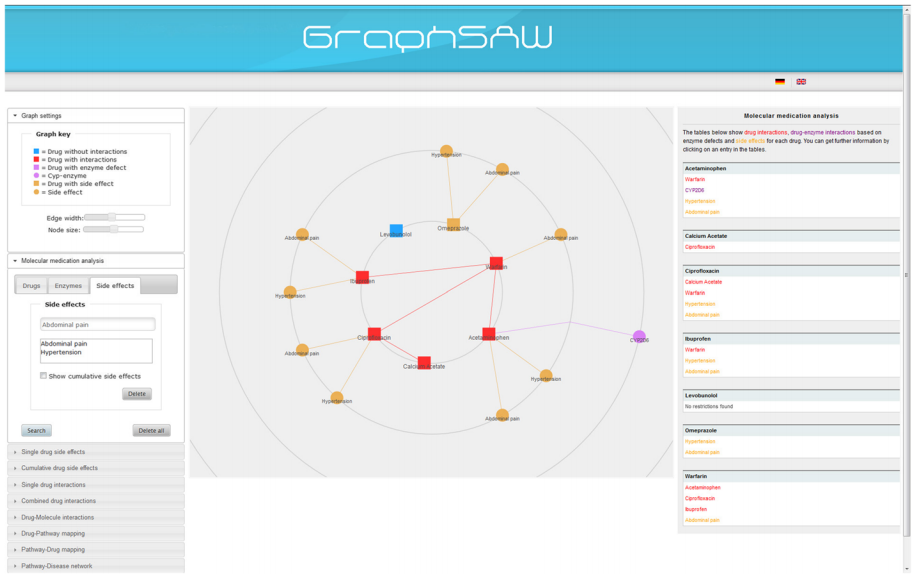
\includegraphics[width=1\textwidth]{fig/litteratursok/graphsaw.PNG}
  \caption{Nettverk av legemiddelinformasjon i Graphsaw. Nettverket viser interaksjoner mellom legemidler (røde noder), interaksjoner mellom legemiddler og enzymer (lilla noder), legemiddelbivirkninger (gule noder) og legemidler uten potensielle risikoer (blåe noder). Til høyre i figuren vises informasjon om nodene og kantene i nettverket \citep{shoshi2015graphsaw}.}
\label{fig:graphsaw}
\end{figure}

\subsection{Elektroniske pasientjournaler}
\acrfull{epj} er en elektronisk samling av registrerte opplysninger om en pasient i forbindelse med helsehjelp. \acrfull{epj} kan brukes for å ta avgjørelser om enkeltpasienter og for å få kunnskap om befolkningen generelt. Løsningene er rettet mot helsepersonell. Per i dag er bruksmønsteret ofte “Skrives én gang, leses aldri” \citep{powsner1994graphical}.  

\acrshort{epj}-systemene som brukes av det norske helsevesenet i dag representerer historiske data for pasienter som fritekst. For å gjøre det enklere å utforske informasjonen og gjøre spørringer i \acrshort{epj} bør innholdet visualiseres og gjøres interaktivt \citep{spense2007information}. Interaksjon kan gi brukeren mulighet til å velge hvordan, og hvilke, data som presenteres. I de neste avsnittene gis eksempler som illustrerer hvordan \acrshort{epj} kan gjøres interaktivt. 

Historiske data kan visualiseres som hendelsesforløp bestående av punkter eller linjesegmenter på en tidslinje. Figur ~\ref{fig:lifeline_timeline} viser hvordan LifeLines\footnote{LifeLines: System for visualisering av personlige legemiddelhistorier utviklet sent på 90-tallet} bruker tidslinjer. LifeLines bruker en visualiseringsteknikk som skiller kategorier av hendelser på separate tidslinjer, og bruker farger for å skille hendelsestypene. 

\begin{figure}[H]
  \centering
    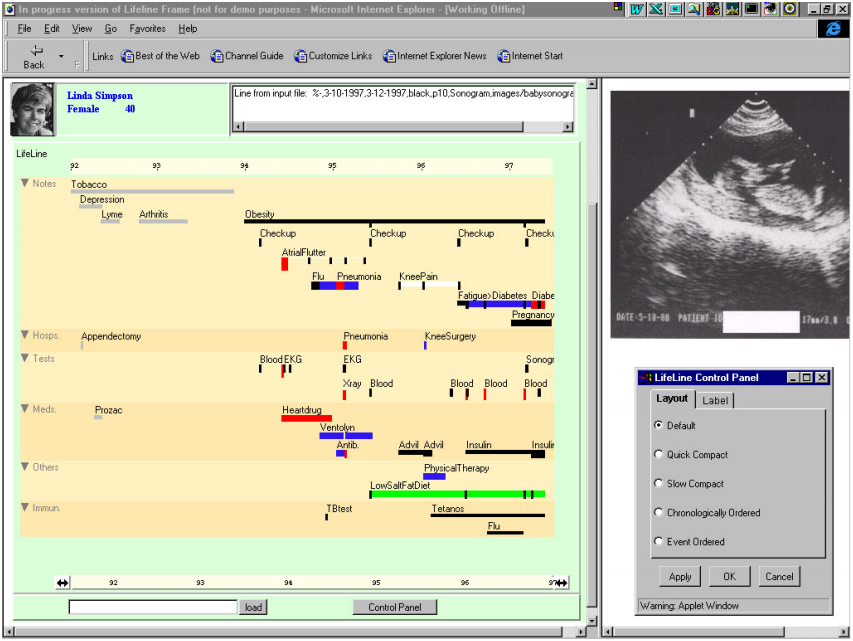
\includegraphics[width=1\textwidth]{fig/litteratursok/lifeline_timeline.PNG}
  \caption{Skjermbilde av bruk av tidslinjer i Lifelines \citep{rind2011interactive}. }
\label{fig:lifeline_timeline}
\end{figure}

LifeLines visualiserte hendelsesforløp for én pasient. Lifelines2 gjør det mulig å se fellestrekk mellom hendelsesforløpene til flere pasienter. Dette gjøres ved å sentrere forløpene rundt en felles hendelse for å få oversikt over hvordan de ulike forløpene har utartet seg før og etter hendelsen det senteres på. Figur ~\ref{fig:lifelines2} viser et skjermbilde fra Lifelifes2 hvor en hendelse representert av gule trekanter er sentrert i bildet. 

\begin{figure}[H]
  \centering
    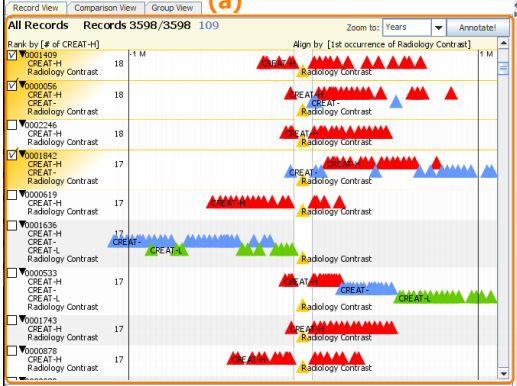
\includegraphics[width=1\textwidth]{fig/litteratursok/lifelines2.PNG}
  \caption{Justering av hendelser i tid mellom pasientforløp i Lifelines2 \citep{rind2011interactive}.}
\label{fig:lifelines2}
\end{figure}

Midgaard\footnote{Midgaard: System for visualisering av behandling på intensivavdelinger} gjør det mulig å endre nivået av detaljer på en tidslinje ved å zoome, se eksempler i figur~\ref{fig:midgaard}. Zoom gir mulighet for personlig tilpasning ved at brukeren selv kan velge detaljerningsnivået på informajsonen som vises \citep{rind2011interactive}. 

\begin{figure}[H]
  \centering
    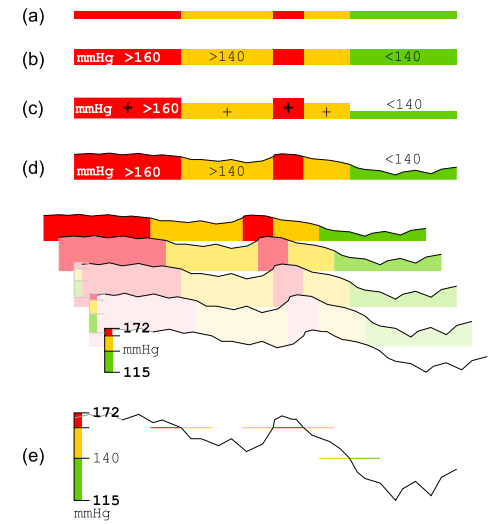
\includegraphics[width=0.6\textwidth]{fig/litteratursok/midgaard.PNG}
  \caption{Viser gradvis økning i detaljnivå ved bruk av zoom i Midgaard \citep{rind2011interactive}}
\label{fig:midgaard}
\end{figure}

Et alternativ til å vise hendelsesforløp som linjer er å bruke ikoner som består av grafiske elementer. Denne måten å visualisere pasientinformasjon på er gjort i et system kalt VIE-VISU\footnote{VIE-VISU: System som visualiserer data fra helseinformasjonssystemer.} som ble tatt i bruk på en intensivavdeling for nyfødte. Hvert ikon representerer helsetilstanden på et bestemt tidspunkt. En serie med 24 ikoner viser utviklingen av pasientens helsetilstand det siste døgnet, som vist i figur~\ref{fig:mange_glyphs}. 

Ikonene består av grafiske elementer som representerer ulike målinger for sirkulasjon, pust og veskebalanse. Størrelsen og fargen på de grafiske elementene brukes til å illustrere målingenes verdi, som vist i figur~\ref{fig:mange_glyphs}. For eksempel er pasientens registrerte puls representert ved bredden på den røde trekanten i hvert ikon.


\begin{figure}[H]
  \centering
    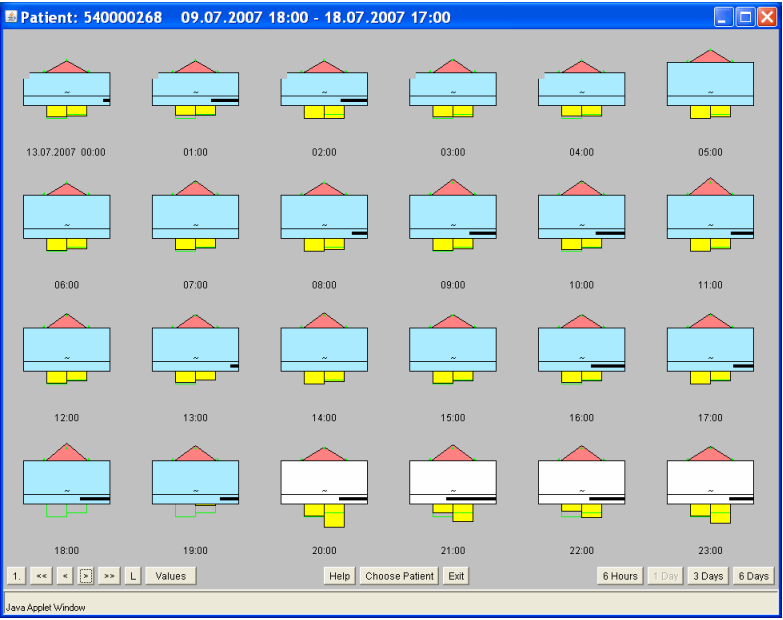
\includegraphics[width=0.6\textwidth]{fig/litteratursok/mange_glyphs.PNG}
  \caption{Bruk av grafiske elementer i VIE-VISU \citep{rind2011interactive}.}
\label{fig:mange_glyphs}
\end{figure}

\begin{figure}[H]
  \centering
    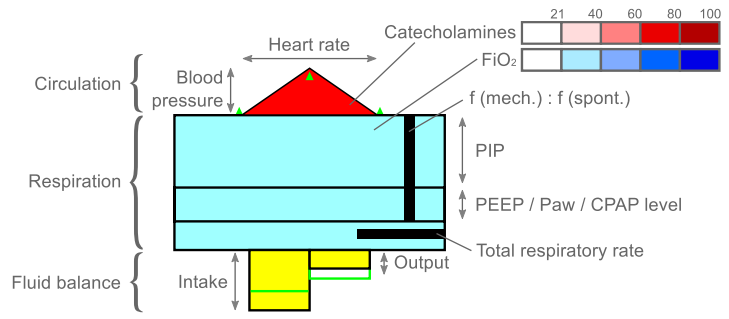
\includegraphics[width=0.6\textwidth]{fig/litteratursok/detalj_glyph.PNG}
  \caption{Bruk av farger i VIE-VISU \citep{rind2011interactive}.}
\label{fig:detalj_glyph}
\end{figure}


\section{Representasjon av legemiddelkunnskap}
Generell legemiddelinformasjon er i stor grad tilgjengelig på Internett. Noe av det som kan skille Mine Medisiner fra eksisterende systemer er personlig og situasjonsavhengig informasjon. For at Mine Medisiner skal være nyskapende bør det kunne svare på spørsmål som krever omfattende søk i eksisterende kilder, eller ekspertise fra helsepersonell, å besvare. For at en ferdig implementasjon av Mine Medisiner skal kunne realiseres må den bygge på en representasjon av legemiddelkunnskap. Vi gjorde et litteratursøk for å undersøke mulighetene for å lage en representasjon av legemiddelkunnskap som egner seg for Mine Medisiner.

For å representere legemiddelkunnskap kan man lage en ontologi. Begrepet ontologi har sin opprinnelse fra filosofien og betegner læren om det som finnes. Innenfor informasjonsteknologi brukes begrepet ontologi for å betegne en formell representasjon av begreper innenfor et domene, og hvordan disse begrepene relaterer til hverandre \citep{barrysmithOnto}.

Et kompetansespørsmål er et typisk spørsmål som man ønsker at en ontologi skal kunne besvare. Kompetansespørsmål definerer ontologiens krav ved at de angir hvilke spørsmål ontologien skal være i stand til å besvare \citep{Gangemi, Fox}.

Kompetansespørsmål kan bli brukt til å vurdere hvor god dekning en ontologi har. Dette gjøres ved at man måler hvor stor prosentandel av kompetansespørsmålene som ontologien er i stand til å besvare. For at kompetansespørsmålene skal gi en god indikasjon på dekningen til ontologien må man sørge for at kompetansespørsmålene i seg selv har god dekning \citep{Rao}.

\begin{table}[H]
    \centering
    \begin{tabularx}{\textwidth}{|X|}
    \hline
        \textbf{Kompetansespørsmål til Mine Medisiner sin ontologi}
        \begin{enumerate}
            \item For enhver effekt skal det være mulig å spørre om et legemiddel eller en kombinasjon av legemidler kan gi denne effekten
            \item For hvert legemiddel skal det være mulig å spørre om legemiddelinformasjon. Legemiddelinformasjon inkluderer:
            \begin{itemize}
                \item Indikasjoner
                \item Mulige bivirkninger
                \item Dosering
            \end{itemize}
            \item For hver legemiddelkombinasjon skal det være mulig å spørre om:
            \begin{itemize}
                \item Interaksjoner  mellom noen av legemidlene i legemiddelkombinasjonen
                \item Overlapp i effekt  mellom noen av legemidlene i legemiddelkombinasjonen
                \item Motvirkende effekter mellom noen av legemidlene i legemiddelkombinasjonen
                \item Om noen av legemidlene i legemiddelkombinasjonen er generiske
            \end{itemize}
            \item Det må være mulig å spørre om indikasjoner, bivirkninger og interaksjoner er relevant for en spesiell pasientgruppe (aldersgruppe, kjønn, livssituasjon o.s.v.) 
        \end{enumerate} \\
    \hline
    \end{tabularx}
    \caption{Kompetansespørsmål til Mine Medisiner sin ontologi}
    \label{tab:kompspm}
\end{table}


En gruppe med fire studenter(HAFE), som tok faget TDT4215 Web Intelligence våren 2015, laget en enkel legemiddelontologi som er hardkodet til å fungere for noen av personene som er presentert i delkapittel~\ref{sec:personae}. Ontologien er i stand til å besvare kompetansespørsmålene til Mine Medisiner sin ontologi (se tabell~\ref{tab:kompspm}), men den inneholder mange forenklinger. Disse forenklingene gjør at ontologien ikke er i stand til å modellere virkeligheten på en tilstrekkelig måte for en ferdig versjon av Mine Medisine. Sluttraporten til HAFE-prosjektet ligger i vedlegg~\ref{HEFE}.

En vanlig kilde til feil i ontologier for legemidler er at virkningen av legemiddelet bare knyttes til enkeltmolekyler av virkestoffer. Virkemidler er viktig for hvilken effekt legemidler får, men også hvilken form (tablett, veske, inhalator) legemiddelet er i, hvilken dose som tas, hvilke andre legemidler som tas, med mer. \acrfull{dron} er en ontologi som tar hensyn til at det er flere faktorer som påvirker effekten av legemidler. \acrshort{dron} har som mål at det skal bli mulig å gjøre spørringer på virkestoff, effekt av legemiddel og den terapeutiske klassen legemiddelet tilhører \citep{HoganTowards, BuildingDrugOntology}.

\acrshort{dron} er avansert, komplekst og muliggjør resonnering, men for at den skal være nyttig for Mine Medisiner må den tilpasses noe i struktur og innhold. \acrshort{dron} må fylles med norske kliniske terminologier (ordnett, \acrshort{icd}10, \acrshort{mesh} og annet fra finnkode.no), og tilpasses så den kan besvare kompetansespørsmålene til Mine Medisiner sin ontologi, se tabell~\ref{tab:kompspm}. 

\acrfull{dideo} er en planlagt ontologi som skal basere seg på \acrshort{dron}, \acrfull{dio} og \acrfull{dinto}. \acrshort{dio} og \acrshort{dinto} er to ontologier for legemiddelinteraksjoner. Fordi \acrshort{dideo} vil inneholde informasjon om interaksjoner vil den kunne besvare flere av kompetansespørsmålene til Mine Medisiner sin ontologi enn \acrshort{dron}. \acrshort{dideo} er imidlertid ikke utviklet enda \citep{brochhausen2014towards}.

KEGG DRUG er en legemiddelinformasjonskilde for godkjente legemidler i Japan, USA og Europa. Legemiddelinformasjonen er strukturert ut i fra kjemiske strukturer og annen informasjon på molekylnivå. Interaksjoner til legemidler som selges på resept i Japan har blitt funnet og lagt til i KEGG DRUG ved å analysere alle pakningsvedlegg ved hjelp av naturlig språkprosessering\footnote{Natural language processing (NLP) er et felt innen informatikk, kunstig intelligens og datalingvistikk som handler om samspillet mellom datamaskiner og menneskelige språks}. Interaksjonene er prosessert og klassifisert i hierarkier av kjemiske strukturer og \acrshort{atc}-koder. Hierarkiene gjør at nettverket av interaksjoner kan analyseres på forskjellige granularitetsnivåer. \acrshort{kegg} DRUG gjør det mulig å søke etter kjente interaksjoner, og forutse potensielle interaksjoner mellom reseptbelagte legemidler i Japan \citep{takarabe2011network}.

For å lage en legemiddelontologi må det ligge en klinisk terminologi til grunn, slik at de som samarbeider som utviklingen har en felles forståelse av konvensjonene for å representere klinisk kunnskap. 

\section{Klinisk terminologi}
Klinisk terminologi betegner ord, uttrykk og begreper brukt i helsevesenet. En utfordring med kilder til legemiddelinformasjon, blant annet pakningsvedlegg, er bruken av vanskelige fagterminologier. I Mine Medisiner er det forsøkt å gjøre innholdet forståelig for folk uten helsefaglig bakgrunn, uten at det skal gå ut over kompletthet eller korrektheten til innholdet. 

Det er både språklige og pragmatiske utfordringer ved å utvikle en medisinsk terminologi. Språket må være riktig og høres naturlig ut for en som snakker språket, og innholdet må passe til oppgavene som skal utføres. En utfordring er at medisinsk terminologi kan avvike fra det som virker logisk eller språklige konvensjoner tilsier, ved at betydningen ikke er ordrett  \citep{rector1999clinical}.

Konsensus omkring medisinske begreper og klassifiseringer har vist seg å ikke alltid være mulig blant klinikere. Begrepet kan ha vidt forskjellig betydning på ulike steder. Dette gjør at lokale tilpasninger er nødvendig for klinisk terminologi. 

Eksisterende medisinske kodeverk, f.eks \acrshort{icd}-10, har en kompleks struktur. Det kan være en utfordring å utvikle kliniske terminologier som tar hensyn til eksisterende kodeverk. En annen utfordring er å holde terminologien oppdatert. En klinisk terminologi må være dynamisk fordi ny informasjon og flere detaljer og relasjoner stadig oppstår. 

Det er viktig å spesifisere hvilke oppgaver terminologien skal støtte, og hvilke aktiviteter og brukere som skal ha nytte av den. En altomfattende terminologi som skal tilfredsstille behovet til både forskere, produsenter, forsikringsselskap, staten og helsetjenesten, er vanskelig å få til. En løsning kan være å lage flere typer terminologier til forskjellig bruk, med SNOMED RT\footnote{SNOMED RT: SNOMED reference Terminology} som referanseterminologi \citep{spackman1997snomed}. 



